% 方法主要分成三個部分

% 介紹一下方法流程
%
\section{方法大綱}
  利用3D點雲環境座內定位,目的主要是為了能夠藉由模擬當時的重建出來的環境,來取得比一般影像定位更多的特徵點資訊。在之前的影像定位研究顯示,只要特徵點的數量越多,代表跟要定位中的照片越多
  的相似處,定位就能夠越準確。整個定位過程分成三大步驟:(1).建置3D點雲環境(2).虛擬照相機設置(3).虛擬影像定位。基於這樣的理由,我們利用 Kinect 紅外深度攝影機這種能夠取得深度的資訊儀器
  幫助我們做出3D的點雲環境。有了3D的點雲環境,透過點雲中的坐標系來作均勻分布(Uniform Distribution),藉由這些有規律的分布區域來決定虛擬照相機的位置。因為每個照相機間距相同,所代表觀察到的區
  域都有固定大小與角度,藉由角度上的調整就可以取得比一般影像定位所照出包涵更廣的角度與更大的覆蓋空間,表示可以取出更好的照片。有了更好的照片,就可以減低之後定位所造成的誤差。圖2-1為整體3D點雲
  環境座內定位的過程,這些流程會在之後章節逐一解釋步驟與這些步驟的目的。
  
%放一張整體的流程圖  
\begin{figure*}
\begin{center}

%[scale=0.5]

  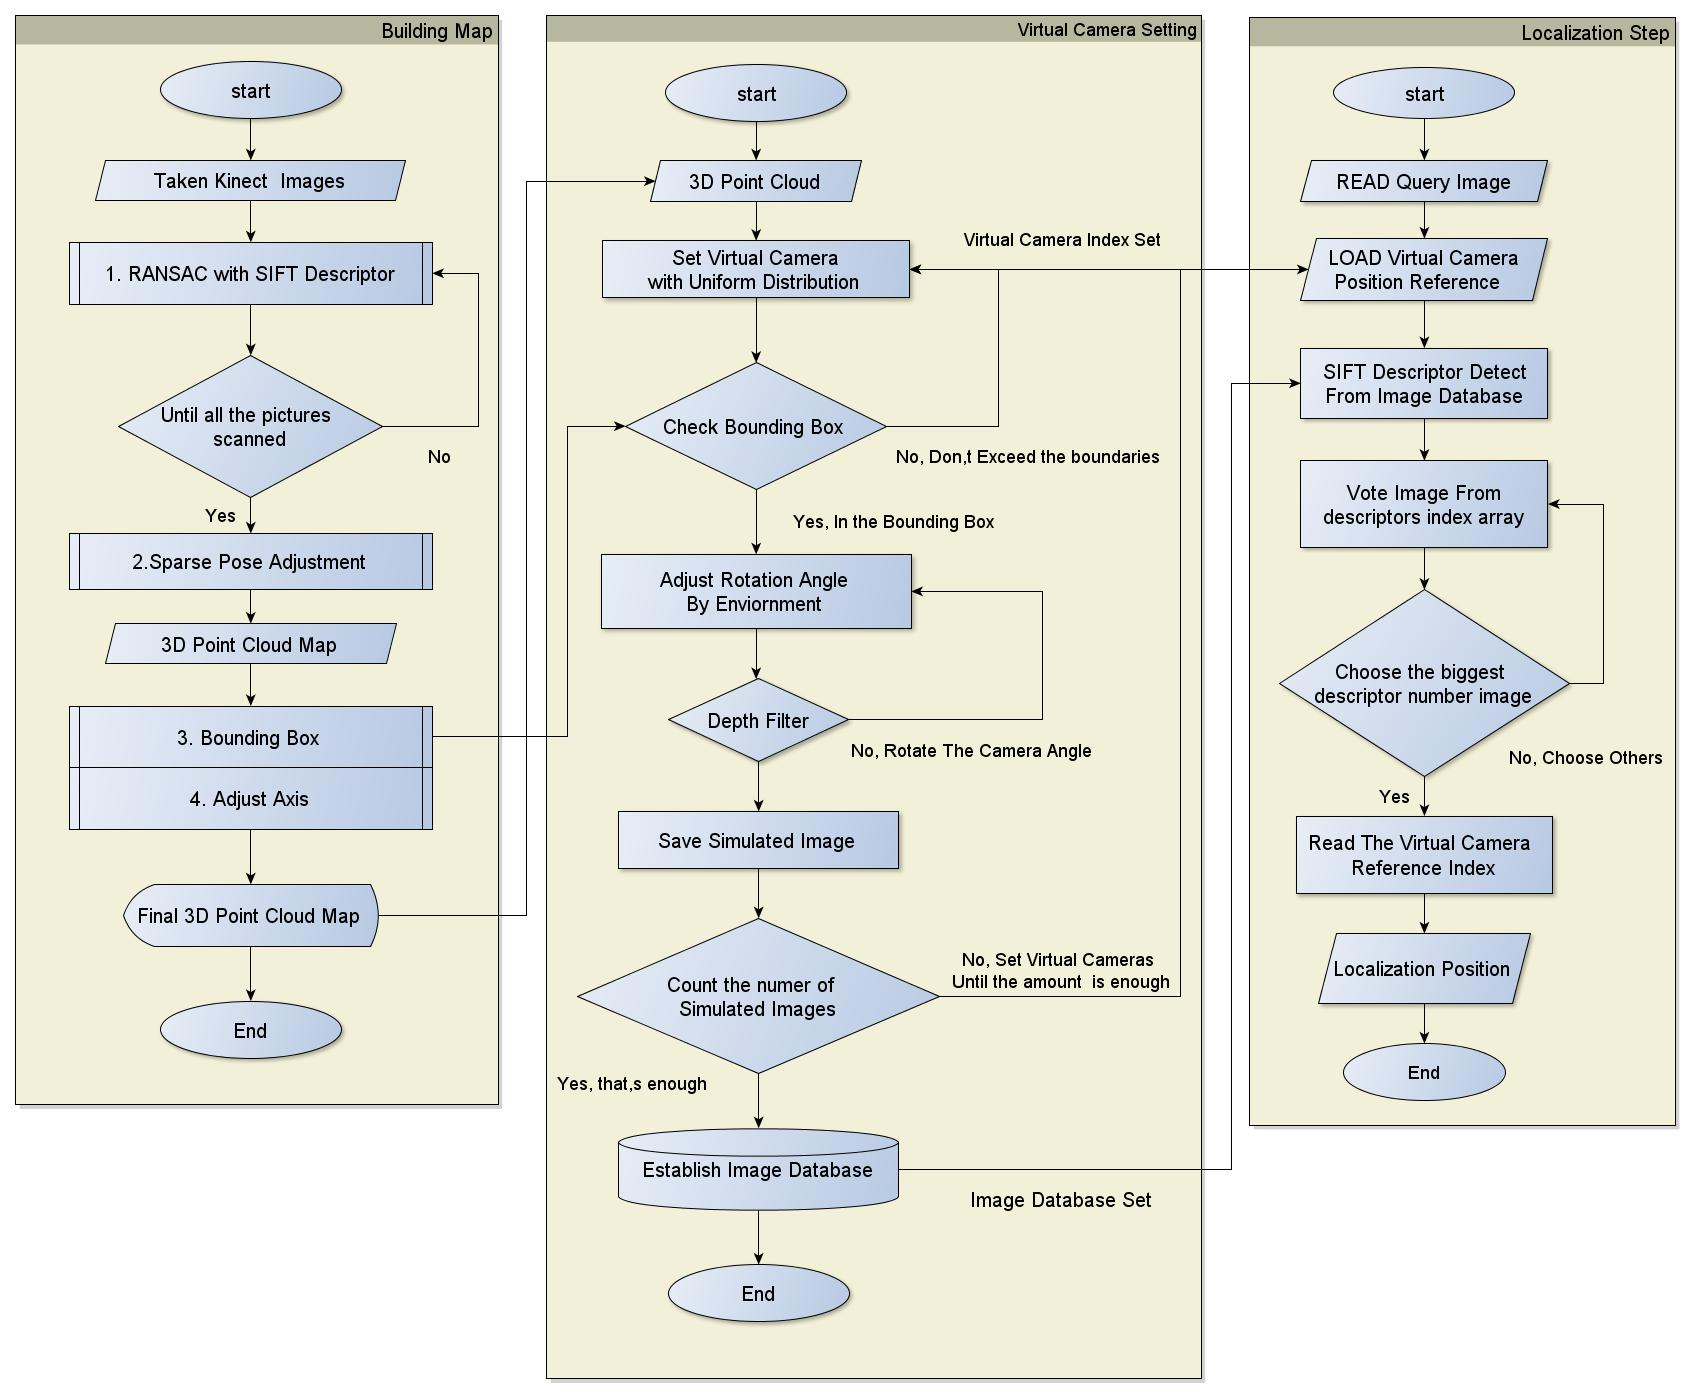
\includegraphics[width=1.1\textwidth]{figures/Enire_System_Process.jpg}
  \caption{3D點雲環境座內定位整體流程圖}
  \label{fig:Enire System Process}

\end{center}
\end{figure*}
  
% 建立 point cloud map
% 
\section{建立3D點雲環境}
   3D環境的建置分成下列五個步驟:

\begin{itemize}
	\item (1) 取得 Kinect 照片
    \item (2) 將偵測到照片中的特徵點作隨機抽樣一致演算法(RANSAC)
    \item (3) 將組好的點雲作Graph SLAM
    \item (4) 設置點雲涵蓋範圍的界線作界限範圍(Bounding Box)
    \item (5) 調整坐標系
\end{itemize}   
   
   前面三個步驟的目的是建置初步的環境,環境有了完整虛擬實境的樣貌後,後面的步驟是為了微調之後撒上虛擬照相機的限制範圍。設限制的區域使虛擬照相機不會放置。在四周看不到任何景物的地方,避免
   製造出沒有使用價值的虛擬相片。接下來將如何製作3D點雲環境分成兩大部分做說明。
   
% 前3個步驟決定點雲的樣子
%
\subsection{虛擬環境的建置}
% Kinect 照片組描述
   一開始先由環境中利用 Kinect 拍攝照片,照片取得的作法類似之前 \cite{Du2011}的方法,在環境上對每個景物做一連串的拍攝,且每張對景物拍攝出來的照片都需要有一些相似之處。環繞整
   個環境的目的是為了不漏掉每個景物。當一個景物越多的環境代表所包含的特徵點越多,擁有豐富的特徵點數量代表之後在做RANSAC可以有更好的效果。像之前在相關研究的章節所述,一個密集的點群所
   找到的平面會越接近真實點群的表現,所做出的 Transformation Matrix 也會越精準,之後重合所做出點雲也會越準,不會有影像疊影或者是無法重合導致點雲中空、物體歪斜扭曲的現象產生
   。連續的環繞拍攝是為了在之後RANSAC的比對有循序的排列,保持每一張影像相對位置關係沒有錯誤。RANSAC 最怕沒有順序的影像排列,沒有順序就沒法找出影像的相對位置,也就是說
   Transformation Matrix 所做出的點雲位置會和實際景物在環境中的位置相差甚遠。拍攝照片在點雲建置的步驟中是影響最大的因素,其中可能光線的不足或是玻璃的反射等一些外在的因素都會導致
   之後在建置點雲的困難,所以在作拍攝時最好都避免這些不利的因素。
     
     
% RANSAC 描述
%   記得找好描述多加一些東西在這  
    有了拍攝的照片組後,利用這些照片取得特徵點的位置,再用這些位置作特徵點求取RANSAC,使得每一張影像都能夠在3D坐標系在對的位置中重合。在這裡使用 MRPT (The Mobile Robot
    Programming Toolkit)的應用程式介面(API),當我們將每張圖片由尺度不辦特徵向量(Scale Invariant Feature Transform)找出來的特徵點作配對,當我們求出來配對關係之後,再將這
    些配對關係作最小平方法(Least Square Error)求出想要的平面,根據不同平面求出 Transformation Matrix ,最後的結果回傳之前照片影像之位置的絕對關係,我們稱為 Global Pose 
    ,Global Pose 包含照片在三維座標以及照片在當時拍攝的角度。Global Pose 在 2D影像定位需要以它作每張影像定位的起始原點,在其他地方像是點雲之後需要調整亦或是找出界限範圍,都需要利
    用 Global Pose 的起始原點當做參考, 但在我們的研究中,我們是使用虛擬相機的 Virtual Camera Pose ,至於 Virtual Camera Pose 的設置方式會在之後詳加說明。有了 Global Pose 
    的位置後,最後我們利用 Graph SLAM 將點雲作最後的調整。
   
    Graph SLAM描述     
          
%放一張初步建好的 3D Point Cloud  和它的 Global Pose

\begin{figure*}
%\begin{center}
  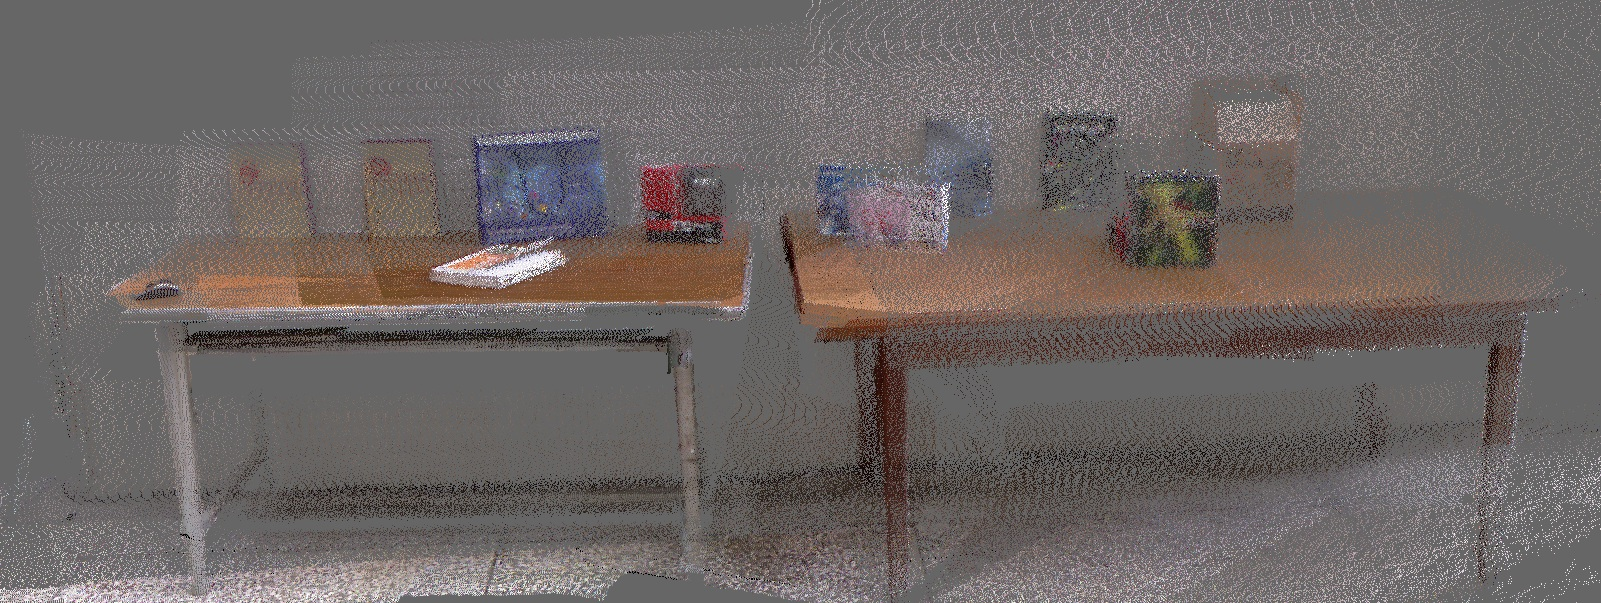
\includegraphics[width=\textwidth]{figures/3DPoint_Cloud_Map.jpg}
  \caption{初步建置好的點雲環境}
  \label{fig:Point Cloud Map}
%\end{center}
\end{figure*}


\subsection{點雲界限範圍制定及大小調整}
     
% 後3個步驟調整點雲分布的界限範圍以及將角度調正
%     
    前三個步驟將點雲完成之後,在之後的過程會將點雲的範圍用 Bounding Box 來制定界線範圍,用照相機的 Global Pose 調整角度。這些目的是為了虛擬照相機能夠在限定的範圍擺放位置,而不使
    有照相機放置在點雲外面,無法產生出有效的虛擬影像作定位。具體的做法如下,當我們讀入整個點雲之後,找出位於坐落在點雲中最大與最小的$X$及$Y$座標,有了這四個座標之後,利用點雲所求
    出的原點,將最大與最小的$X$及$Y$座標互相相減,所求出的長度即為 Bounding Box 的長寬。有了這些長度之後,就可以知道整個點雲或者是說環境的長寬距離為多少,在之後可以防止虛擬照相
    機坐落在散布點雲以外的位置。

%放有 Bounnding Box 的 Point Cloud 圖  

\begin{figure*}
\begin{center}
  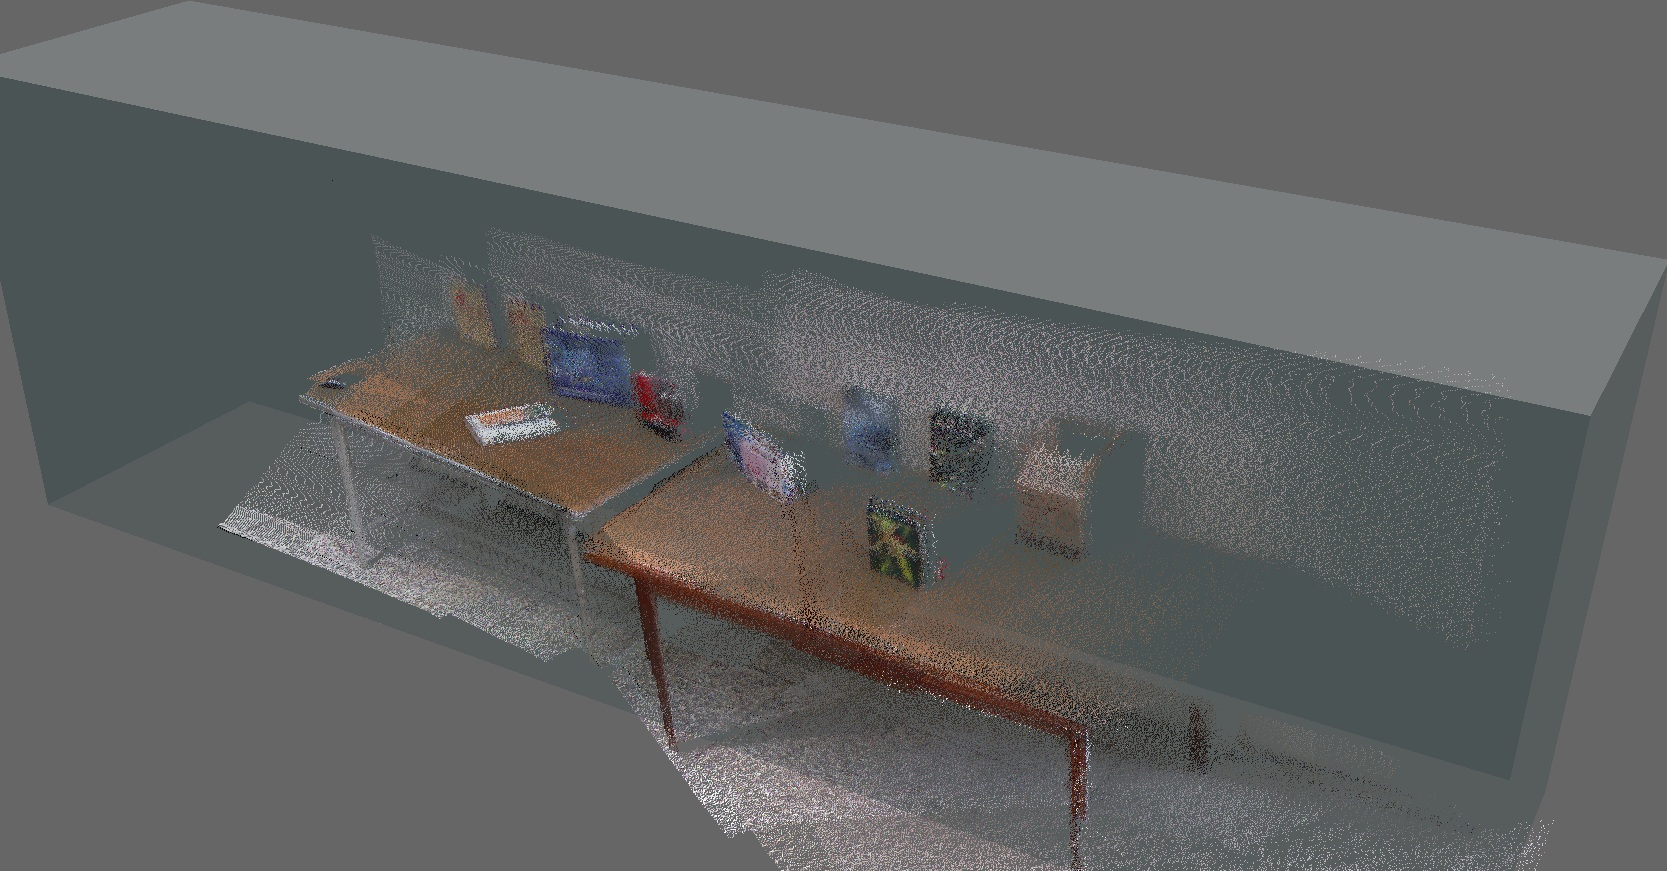
\includegraphics[width=0.5\textwidth]{figures/Bounding_Box.jpg}
  \caption{將點雲給予界限範圍}
  \label{fig:Bounding Box}
\end{center}
\end{figure*}   
    
    知道界限範圍之後,做出來的點雲可能會因為之前Kinect攝影機的 Global Pose 歪斜分布而使得點雲也會有歪斜的狀況產生,這時候就必須將點雲作角度上的調整。這個步驟是為了之後的虛擬相機在照相時
    不會因點雲角度歪斜而使得照出來的角度與真實相機的角度差異過大,減少許多對應的特徵點,導致定位的誤差產生。具體的做法先看出點雲分布的情況是往哪個方向歪斜,利用 Global Pose 來算出
    兩個Kinect攝影機角度的 $\tan \theta$,求出 $\theta$ 之後,將每個點雲帶入旋轉矩陣利用算出來的$\theta$將每個點旋轉至與座標軸平行的角度。調整完正確地角度之後,點雲的界線範圍與旋轉角
    度都與座標軸方向一致後,就可以準備虛擬相機的準備工作。

    
%放一張 攝影機 Global pose 求得後放置旋轉矩陣 的圖   
%放調整角度前的 Point Cloud 與調整角度後 Point Cloud 圖  
    
\begin{figure}
  \begin{center}
    \subfigure[使用攝影機的Global Pose求得$\tan \theta$]{\label{fig:tan}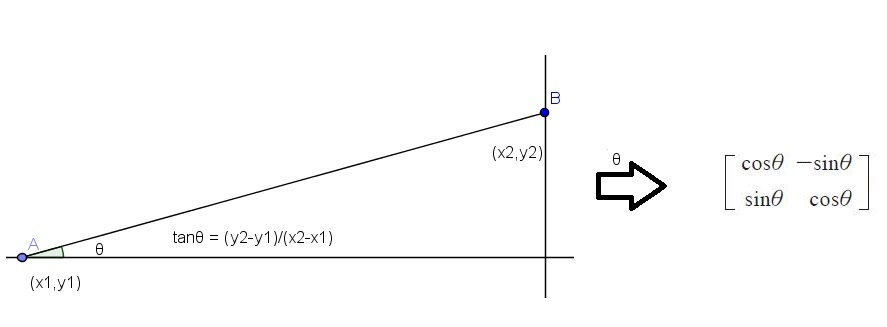
\includegraphics[width=0.65\columnwidth]{figures/Global_Pose.jpg}}
    \subfigure[坐標軸角度差異]{\label{fig:rotation result}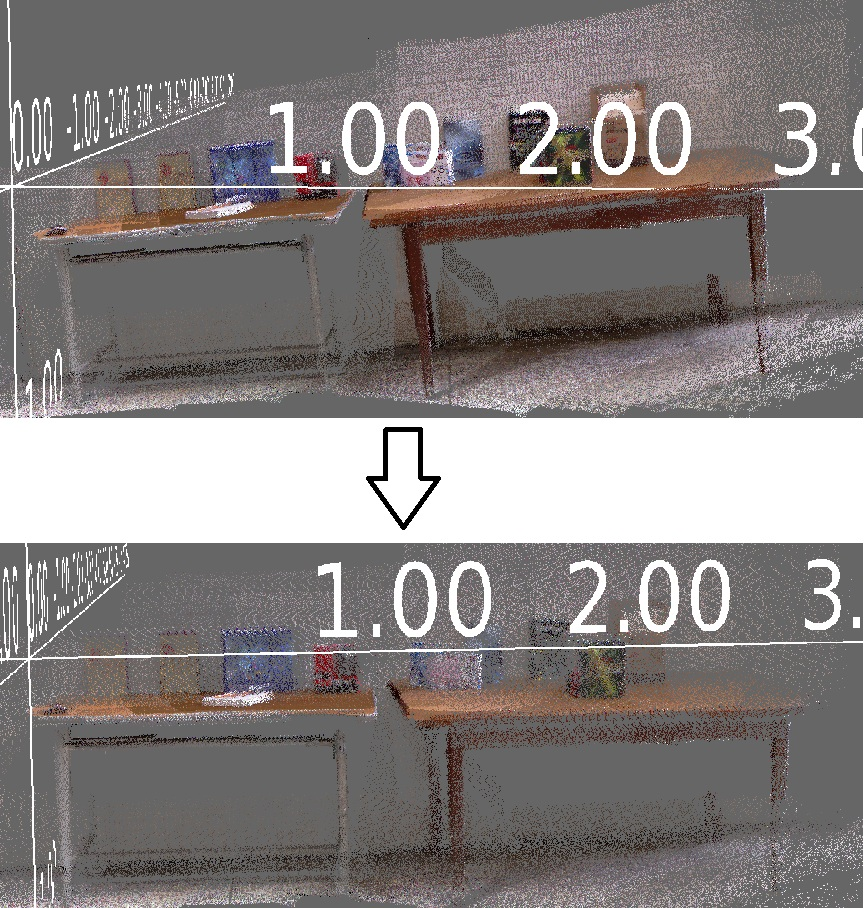
\includegraphics[width=0.33\columnwidth]{figures/Rotation_Result.jpg}}
  \end{center}
  \caption{調整點雲坐標軸角度方法 }
  \label{fig:rotate axis}
\end{figure}
    
\section{虛擬照相機設置及影像資料庫建置}
	
	在建置完環境之後,接下來利用這個章節來描述如何決定虛擬照相機的位置、角度以及虛擬照相機成像的原理。與一般2D影像定位方法不同的是,傳統的2D影像定位內的影像資料庫,大部分都是利用隨機位置
	取得影像資料,而在我們的作法是先利用均勻分布(Uniform Distribution)設置虛擬照相機的位置,再利用隨機分布的角度來決定照相機拍攝的角度。依照這樣的作法,我們能取得比一般影像定位更多的
	環境資訊,而這些資訊都是利用點雲所產生的,不必再額外人工存取kinect攝影機的影像資料,我們所要輸入的資料只需要點雲就可以了。之後我們將分成四個部分描述虛擬照相機的設置:
	
	\begin{itemize}
		\item (1) 均勻分布設置虛擬攝影機
    	\item (2) 虛擬照相機成像原理
    	\item (3) 根據深度來調整攝影機角度
    	\item (4) 儲存虛擬照相機圖片
	\end{itemize}  		

\subsection{均勻分布設置虛擬攝影機}
%均勻分布設置虛擬攝影
%
	上一個章節中,我們完成了實驗環境的建置,也就是點雲的資料,將點雲切割成數等分的區塊,每個區塊都設置一個虛擬照相機,目的為了環境內每個景物都有充分去拍攝而取得足夠的特徵點。作法依據環境而
	有所改變,首先將長分成8個等分、寬分成7個等分,這樣每個等分都會有一樣的距離間隔。在每個間隔放置虛擬照相機,接下來再隨機分布照相機角度,完成虛擬照相機布置的工作。隨機分布照相機角度比一般
	2D影像定位所建置的資料庫比較有更寬廣的角度。一般影像資料庫可能只針對特定區域的特徵點作取樣,而導致特定區域內的影像定位效果非常好,但在其他區域卻沒有足夠的影像特徵點資料,使得定位誤差範
	圍過大,透過均勻分布不會有部分景物或場景沒有被拍攝到,也可以增加定位的覆蓋率。
	
	\begin{figure*}
	\begin{center}
	  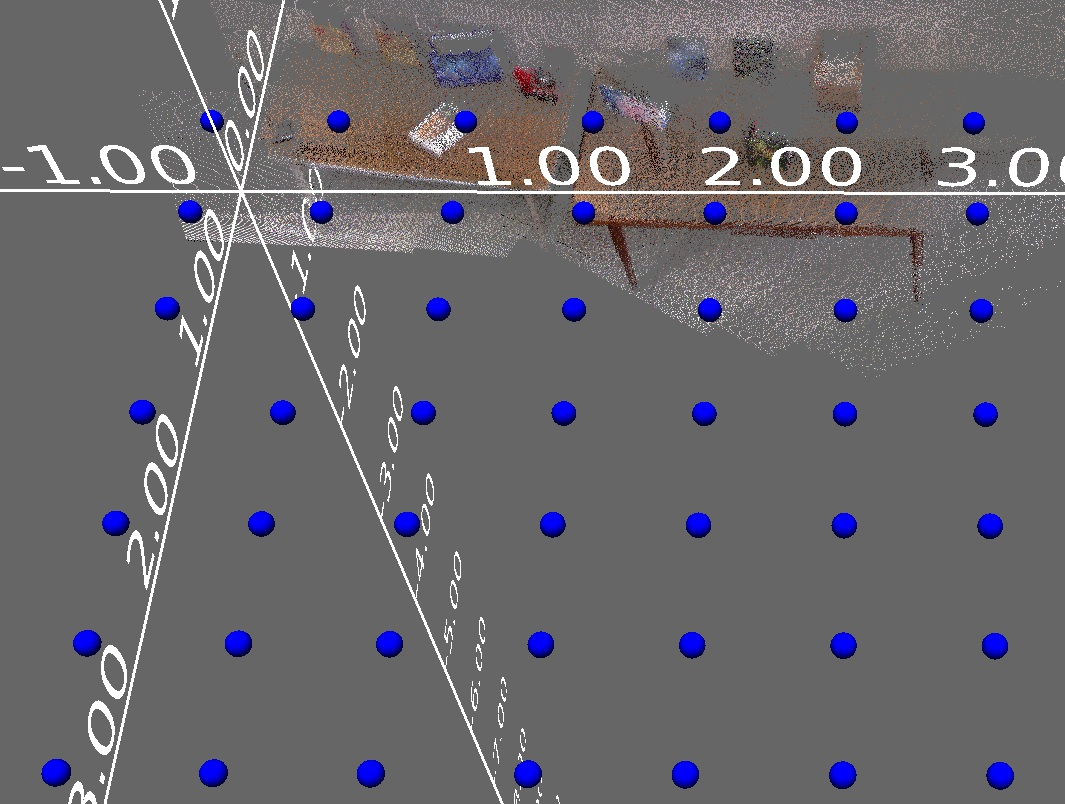
\includegraphics[width=0.5\textwidth]{figures/VirtualCameraPose.jpg}
	  \caption{在點雲上設置虛擬照相機位置}
	  \label{fig:Virtual Camera Pose}
	\end{center}
	\end{figure*}
	


\subsection{虛擬照相機成像原理}
%虛擬照相機成像原理
%
	當虛擬相機位置固定之後,接下來利用虛擬相機拍攝照片,虛擬相機主要由OpenGL這套API來實作,透過攝影機的影像角錐來模擬相機的成像,將角錐內3D影像投影成2D影像,模擬照相機所照出的照片。
	在OpenGL的坐標系,先將視野調整到虛擬照相機的位置,再利用glFrustum 的矩陣取得相機影像角錐,這個矩陣目的在於模擬相機光線經過透鏡成像,在投影到平面影像呈現看出來的照片,矩陣表示法如
	下:
	
	\begin{align}
	glFrustrum = \left(
		 			\begin{array}{cccc}
		 			\frac{2near}{right - near} & 0 & \frac{right + left}{right - left} & 0 \\
		 			0 & \frac{2near}{top - bottom} & \frac{top + bottom}{top - bottom} & 0 \\
		 			0 & 0 & \frac{far + near}{far - near}  & \frac{2far \times near}{far - near} \\
		 			0 & 0 & -1 & 0 \\
		 			\end{array}
		 		\right)
	\end{align}
	
	                    
	將座標轉為齊次座標後,利用攝影機的攝影近裁面(near)與遠裁面(far)的相似三角形來推出這個矩陣,這個矩陣會將角錐內的景像投影到2D平面上,即可完成虛擬照相機的建置。這部分攝影機的焦距設定,
	以及解析度都參照Kinect紅外深度攝影機的參數設定。與真實相機的相機參數相同,再接下來實驗就相機拍出來的照片作對照,做為比較的依據。當我們截取下攝影機的圖片後,會先將角錐內影像的深度作平
	均,為的是求取平均深度來看虛擬相機取的位置會部會太逼近虛擬環境內的景物,或是虛擬相機位置太靠近點雲邊界,這部分會在之後的章節作說明。
	
	\begin{figure*}
	\begin{center}
	  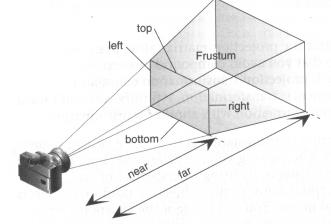
\includegraphics[width=0.5\textwidth]{figures/Camera_image.jpg}
	  \caption{攝影機的攝影近裁面(near)與遠裁面(far)表示}
	  \label{fig:glFrustum}
	\end{center}
	\end{figure*}	

\subsection{根據深度來調整攝影機角度}
%根據深度來調整攝影機角度
%

	\begin{figure*}
	\begin{center}
	  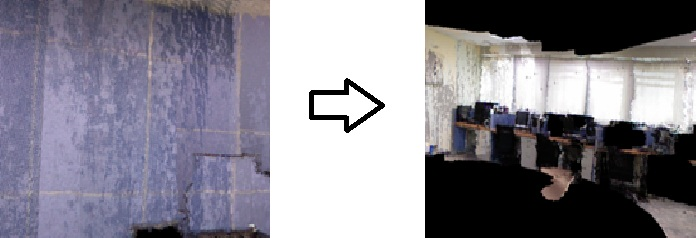
\includegraphics[width=1.0\textwidth]{figures/Depth_Filter.jpg}
	  \caption{根據物體距離鏡頭遠近來調整方位}
	  \label{fig:Depth_Filter}
	\end{center}
	\end{figure*}

	當虛擬照相機的圖片擷取出來後,因為拍照的相機深度過淺,而導致拍攝的景物無法辨識,這時候我們利用深度過濾的機制來將照相機取得角度作過濾。一般深度buffer分為z-buffer與w-buffer兩種,
	先從兩種不同的深度分辨方式作探討:
	
	首先作關於深度的計算,利用四維座標軸$(x,y,z,w)$表示三維座標軸$(x',y',z')$的點,空間關係的表示法為:
	\begin{align}
		\left\{
		\begin{array}{ccc}
		x' = x /w \\
		y' = y /w \\
		z' = z /w \\
		\end{array}
		\right.
	\end{align}
	
	根據figure 2-6的示意圖表示,$Z_n = near$面的z範圍,$Z_f = far$面z範圍,$w = \frac{2 \times Z_n}{right-left}$,$Q = \frac{Z_f}{Z_f - Z_n}$ 所以由z座標求得w縮
	放的比例,式子可以寫為:
		
	\begin{align}
		w = \frac{Q\times Z_n}{(Q-Z)}
	\end{align}			
	
	z-buffer 是保存經過glFrustrum投影變換後的 z 坐標,投影後物體會產生近大遠小的效果,所以距離眼睛比較近的地方,z 坐標的分辨率比較大,而遠處的分辨率則比較小。換句話說,投影後的
    z 坐標在其值得分布上,對於景物對眼睛的物理距離變化來說,不是線性變化的(即非均勻分佈),這樣的一個好處是近處的物體得到了較高的深度辨識,但是遠處物體的深度判斷可能會出錯。 
    
    w-buffer 保存的是經過投影變換後的齊次坐標系中的 w 坐標,而 w 坐標通常跟世界坐標系中的 z 坐標成正比,所以變換到投影空間中之後,其值依然是線性分佈的,這樣無論遠處還是近處的物體,都
    有相同的深度分辨率,這是它的優點,當然,缺點就是不能用較高的深度分辨率來表現近處的物體。
    
    針對兩種不同的深度Buffer比較,因為我們的做法是來判別景物是否距離鏡頭過近,所以在深度判斷上是採用z-Buffer的作法,當我們判斷鏡頭與物體距離實際深度小於80公分時,我們會將照相機鏡頭角度
    轉向180度,也就是正後方來重新拍攝。
    

\subsection{儲存虛擬照相機圖片}
%儲存虛擬照相機圖片
%
	當已經決定取好的照片之後,利用虛擬照相機將取出的照片來儲存至影像資料庫,來進行接下來定位的前置作業。虛擬影像儲存是透過虛擬照相機鏡頭裡的每一個pixel寫入相片裡頭,主要做法如下。當從 
	z-buffer 讀出來的深度錯誤時,代表這個 pixel 對應在點雲上是一個黑點或者是說根本沒有點雲的資訊,則以黑色為代表,當深度沒影錯誤時,則代表它具有實際點雲的資料,我們找出點雲對應點的
	顏色資訊,寫入圖檔裡,這樣即可完成初步的虛擬相片。根據上述的方法,還會遇到透視的問題,就是說原本不應該出現的景物因為深度有誤差,而原本在障礙物之後的物體卻跑在障礙物之前,像是穿透障
	礙物一樣,例如 figure 2-9 原本不該出現桌子的地方,因為發生了透視的現象而出現了桌子。改進方法為根據周圍的深度來做內插補強。
	
%放一個內插補強前後的差異圖	
	\begin{figure*}
	\begin{center}
	  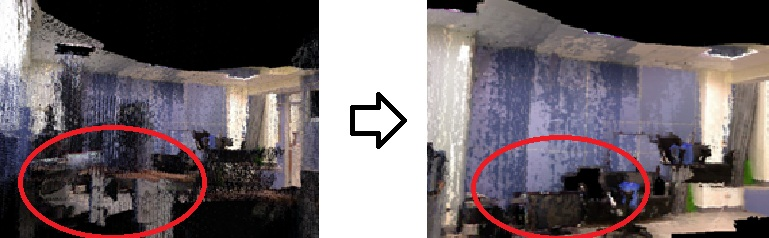
\includegraphics[width=1.0\textwidth]{figures/Depth_Interpolation.jpg}
	  \caption{內差法補強前後的差異圖}
	  \label{fig:interpolation}
	\end{center}
	\end{figure*}	
	
	虛擬影像的資料量因環境而變,主要根據 Global Pose 在每個位置上取出相隔120度的兩個不同角度的相片,在一般情況下環境中取出 50 點的 Global Pose ,所以總共會有 100 張的虛擬相片
	。藉由這些虛擬相片,我們取得了環境所在內的不同位置與不同角度的資料,比起一般的影像定位資料多出了更豐富的特徵點資訊。之後的實驗可以比較出來,在不同位置以及距離特徵點的遠近對定位會帶
	來什麼樣的影響。到了最後定位的流程,將介紹虛擬影像的定位方法。

\section{虛擬影像定位}

% 定位的決策
%
	在定位的流程中,利用讀取要定位的圖片,根據定位照片的特徵點比較找出最合適的虛擬影像,再參照虛擬影像所在的虛擬照相機的位置來定位。這樣可以節省利用三角定位(Triangulation)的時間,
	根據之前不同的影像資料庫的建置方法,又增加許多以前傳統影像定位所定位不到的地方,關於這種覆蓋率的數據比較,在之後的實驗方法有詳細的數據可以佐證增加覆蓋率的證明。
	
	在定位的程序上,主要會分成3個階段:
		\begin{itemize}
			\item (1) 前置作業處理
    		\item (2) 尋找特徵點並找出最多的特徵點投票選出位置
    		\item (3) 利用虛擬照相機位置來定位
		\end{itemize} 
	
	
\subsection{前置作業處理}	
%前置作業處理

	在定位之前,先輸入待定位的照片以及虛擬照相機的位置。虛擬照相機的位置記錄檔格式包含每個虛擬相機的$X,Y,Z$座標以及每個攝影機的角度位置,當流程步驟做到特徵點定位時,就會需要參考到
	虛擬相機的位置。
		
\subsection{尋找特徵點並找出最多的特徵點投票選出位置}	
%尋找特徵點並找出最多的特徵點投票選出位置

	在前置作業完成之後,接下來利用所有資料庫中的照片進行比對,並將每張照片所擁有找到與被定位照片相同的特徵點數量記錄下來。在這裡使
	用的的方法為尺度不辨特徵向量(Scale Invariant Feature Transform),簡稱為SIFT,我們利用SIFT找出與相片中相同的特徵點,
	並將找出的特徵點的數量給記錄下來。關於SIFT的作法在之前已經有了相關的敘述,所以可以得知當存在虛擬相片中特徵點的數量越多,代表與
	所要定位的照片有越密切的關係,當我們在所有照片中選出來擁有最多特徵點數量的虛擬照片時,我們參考這個拍攝虛擬照片的相機的編號,根據
	編號找出相機所在的位置,再利用這個虛擬相機的pose當作初步所在定位的定位位置。
	
	\begin{figure}
    	\begin{center}
    		\subfigure[根據虛擬相片找出的特徵點]{\label{fig:SIFT_Descriptor}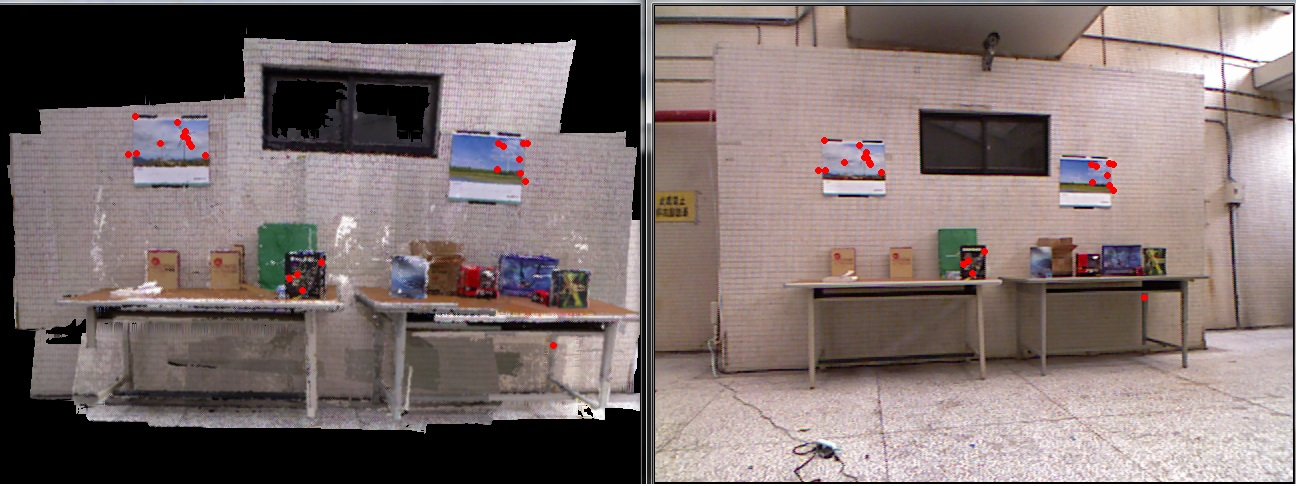
\includegraphics[width=1\columnwidth]{figures/SIFT_Descriptor.jpg}}
    		\subfigure[根據實際相片找出的特徵點]{\label{fig:SIFT_Descriptor2}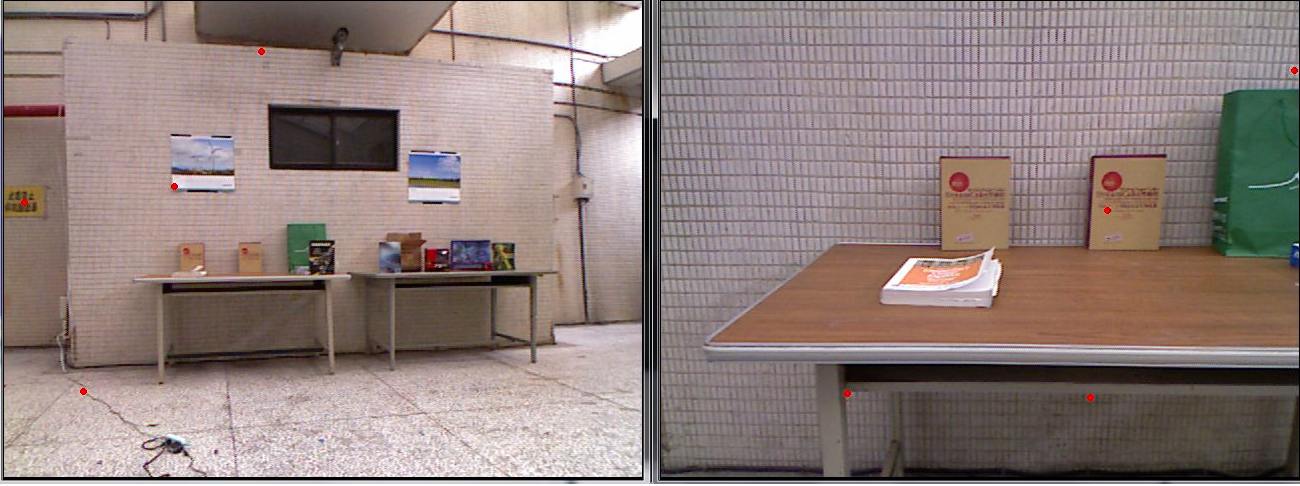
\includegraphics[width=1\columnwidth]{figures/SIFT_Descriptor(2).jpg}}
    	\end{center}
    	\caption{特徵點比較差異圖 }
    	\label{fig:SIFT_Descriptor}
    \end{figure}
	
	特徵點的分布跟環境景物的分布有密切的關係,在我們的作法上藉由虛擬照片找到距離特徵景物遠的待定位照片,卻可以比一般的照片找出更多的特徵點。利用虛擬照片我們可以有效的找出更多的環境特
	徵,在之後的定位上不管是覆蓋率或是精準度都有一定程度的提升。

\subsection{利用虛擬照相機位置來定位}
%利用虛擬照相機位置來定位

	最後定位我們利用虛擬相機的位置來當作定位的參考位置,在利用虛擬相機的位置來定位與一般影像定位不同的地方在於三角定位的使用。在這裡我們先解釋一般三角定位的流程:
	\begin{itemize}
			\item (1) 找出特徵點對於鏡頭的夾角
    		\item (2) 利用夾角帶入餘弦定理(Cosine Law)求出特徵點所距離鏡頭位置的長度
    		\item (3) 利用已知的長度求出待定位圖片的位置
	\end{itemize}
	
	\subsubsection{找出特徵點對於鏡頭圖片的夾角}
	
	\begin{figure*}
	\begin{center}
	  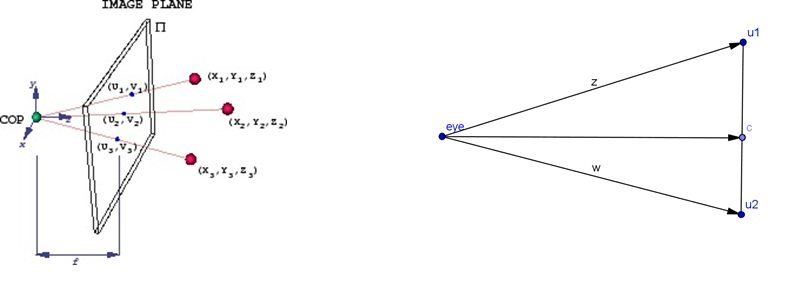
\includegraphics[width=1.0\textwidth]{figures/Included_Angle.jpg}
	  \caption{相機與特徵點的夾角示意圖}
	  \label{fig:Included Angle}
	\end{center}
	\end{figure*}
	
	在 \ref{fig:Included Angle} 當中我們要先求得$\vec{z}$與$\vec{w}$的長度,當我們知道$\vec{U_1}$與$\vec{U_2}$之後,帶入下列求解的算式:
	\begin{align}
		\left\{
		\begin{array}{cccc}
		\vec{z} = (u_{1x} - c_x)\vec{u} + (v_{1y} - c_y)\vec{v} + \vec{f}d\\
		\vec{w} = (u_{2x} - c_x)\vec{u} + (v_{2y} - c_y)\vec{v} + \vec{f}d\\
		\end{array}
		\right.
	\end{align}
	在這之中,f 為焦距向量,d 為深度。	
	
	我們得到$|z|$與$|w|$的長度,在 fig:2-11 我們知道$|u|$的長度之後,再帶入餘弦定理求得角度$\alpha$的夾角:
	\begin{align}
		|\vec{u}|^2 = |\vec{z}|^2 + |\vec{w}|^2 - 2zwcos\alpha
	\end{align}	
	
	\subsubsection{利用夾角帶入餘弦定理 (Cosine Law) 求出特徵點所距離鏡頭圖片位置的長度}
	
	\begin{figure}
    \begin{center}
    		\subfigure[角度$\alpha$對於夾角$\vec{z}$與$\vec{w}$示意圖]{\label{fig:Included Angle(2)}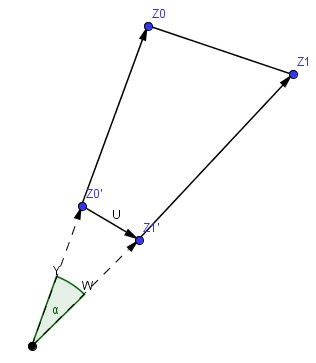
\includegraphics[width=0.3\textwidth]{figures/Included_Angle(2).jpg}}
    		\subfigure[利用夾角帶入餘弦定理 (Cosine Law) 求出特徵點所距離鏡頭圖片位置的長度]{\label{fig:Localization}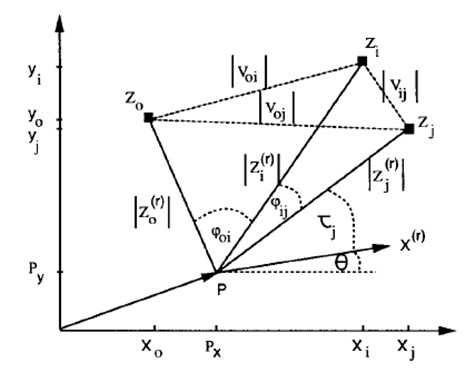
\includegraphics[width=0.6\textwidth]{figures/Localization.jpg}}
    \end{center}
    \caption{定位點夾角與長度向量關係示意圖}
    \label{fig:Localization Relationship}
    \end{figure}


	由 \ref{fig:Localization Relationship} 我們可以知道$\varphi _{oi}$與$\varphi _{ij}$也知道$|V_{oi}|$, $|V_{oj}|$與$|V_{ij}|$的長度,藉由餘弦定理可以推出下列算式:
	
	\begin{align}
		\left\{
		\begin{array}{cccc}
		|V_{oi}|^2 = |Z_o^{(r)}|^2 + |Z_i^{(r)}|^2 - 2|Z_o^{(r)}||Z_i^{(r)}|\varphi _{io}\\
		|V_{oj}|^2 = |Z_o^{(r)}|^2 + |Z_j^{(r)}|^2 - 2|Z_o^{(r)}||Z_j^{(r)}|\varphi _{jo}\\
		|V_{ij}|^2 = |Z_i^{(r)}|^2 + |Z_j^{(r)}|^2 - 2|Z_j^{(r)}||Z_j^{(r)}|\varphi _{ij}\\
		\end{array}
		\right.
	\end{align}	
	
	其中(r)代表從定位點 P 所觀測出的位置與視角。	
	
	當我們解出$|Z_o|$,$|Z_i|$以及$|Z_j|$之後,根據圖上的座標表示法,我們最後帶入式子(2.7)中求解
	
	\subsubsection{利用已知的長度求出待定位圖片的位置}
	
	\begin{align}
		\left\{
		\begin{array}{cccc}
		|Z_o^{(r)}| = (x_o - p_x)^2 + (y_o - p_y)^2\\
		|Z_i^{(r)}| = (x_i - p_x)^2 + (y_i - p_y)^2\\
		|Z_j^{(r)}| = (x_j - p_x)^2 + (y_j - p_y)^2\\
		\end{array}
		\right.
	\end{align}	
	
	我們利用上述式子整理可得出下列式子:
	
	\begin{align}
		\left\{
		\begin{array}{cccc}
		|Z_o^{(r)}|^2 - |Z_i^{(r)}|^2 = X_o^2 - X_i^2 + 2p_x(x_i - x_o) + y_o^2 - y_i^2 + 2p_y(y_i-y_o)\\
		|Z_o^{(r)}|^2 - |Z_j^{(r)}|^2 = X_o^2 - X_j^2 + 2p_x(x_j - x_o) + y_o^2 - y_j^2 + 2p_y(y_j-y_o)\\
		\end{array}
		\right.
	\end{align}	
	
	在依照(2.7)式子兩兩相減,可得出六項聯立方程組,(2.8)為其中的兩項,在式子當中我們求出$p_x$及$p_y$則為我們想要定位之座標。
	
    上面為傳統2D平面影像根據特徵點的定位流程,我們根據虛擬影像也可以與待定位照片根據特徵點定位。但是虛擬影像為3D投影回2D的平面影像,在座標空間表示
    會面臨到投影所產生的誤差,再者點雲所見出的環境深度因為Kinect深度攝影機本身偵測的深度也會產生誤差,由虛擬影像跟平面影像特徵點利用式子求解比平面
    影像定位求解來的誤差更大。根據這點,我們利用虛擬相機的位置來當參考的定位點,當我們找出最多特徵點的虛擬照片後,我們還是利用虛擬影像作三角定位,當
    所求的定位點與虛擬相機絕對距離超過70公分,我們就利用虛擬相機位置做最後定位點,否則則三角定位的位置則為最後定位完成的結果。
    
    會這樣做的理由基於我們每個相機的x軸距離與y軸距離是50公分,為均勻分布,所以假定最大的平均定位誤差就為$\sqrt{x^2+y^2}=70.7$公分,當定位超過
    這個平均誤差距離,我們最後還是捨棄三角定位的結果,改以最多特徵點的虛擬相機位置為最終的成果。
